\documentclass[conference]{IEEEtran}
\pdfpagewidth=8.5in
\pdfpageheight=11in
%\usepackage{subfig}
\usepackage{subfigure}
\usepackage[pdftex]{}
\usepackage{graphicx}
%\usepackage{todonotes}
\usepackage{listings}
\lstset {% general command to set parameter(s)
         language=C,
     basicstyle=\footnotesize,               % print whole listing small
%     keywordstyle=\color{black}\bfseries, % underlined bold black keywords
%     identifierstyle =\color{black},  % nothing happens
%     commentstyle=\color{black}\emph, % white comments
     %stringstyle=\ttfamily,          % typewriter type for strings
%     stringstyle=\color{black},       % typewriter type for strings
         tabsize=4,
         showtabs=false,
     showstringspaces=false}
%can't figure this one out for particles bandwidth
%\usepackage[caption,label]{subfig}

%\newcommand{\TITLE}{D\textsuperscript{\huge{2}}T: Doubly Distributed Transactions for High Performance and Distributed Computing}

\newcommand{\DDT}{D\textsuperscript{2}T~}
\newcommand{\DDTns}{D\textsuperscript{2}T}

\hyphenation{sub-trans-ac-tion}

\addtolength{\parskip}{-0.08in}

% in order for balance columns to work, it has to be before begin document...
%\balancecolumns

\begin{document}

%\conferenceinfo{Cluster'14,} {September 17, 2014, Madrid, Spain}
%\CopyrightYear{2014}
%\crdata{978-1-4503-1103-8/11/11}
%\clubpenalty=10000
%\widowpenalty = 10000

\title{An Innovative Storage Stack Addressing Extreme Scale Platforms and Big Data Applications}

\author{
\IEEEauthorblockN{Jay Lofstead\IEEEauthorrefmark{1}, Ivo Jimenez\IEEEauthorrefmark{2}, Carlos Maltzahn\IEEEauthorrefmark{2}, Quincey Koziol\IEEEauthorrefmark{3}, John Bent\IEEEauthorrefmark{4}, Eric Barton\IEEEauthorrefmark{5}}
\IEEEauthorblockA{\IEEEauthorrefmark{1}Sandia National Laboratories gflofst@sandia.gov}
\IEEEauthorblockA{\IEEEauthorrefmark{2}University of California, Santa Cruz ivo@cs.ucsc.edu, carlosm@soe.ucsc.edu}
\IEEEauthorblockA{\IEEEauthorrefmark{3}HDF Group koziol@hdfgroup.org}
\IEEEauthorblockA{\IEEEauthorrefmark{4}EMC john.bent@emc.com}
\IEEEauthorblockA{\IEEEauthorrefmark{5}Intel eric.barton@intel.com}
}
\maketitle

\begin{abstract}
The DOE Extreme-Scale Technology Acceleration Fast Forward Storage and IO Stack
project is going to have significant impact on storage systems design within
and beyond the HPC community. With phase 1 of the project complete, it is an
excellent opportunity to explore the complete design and how it will address
the needs of extreme scale platforms.  This paper examimes the overall design.
Each layer of the proposed stack is discussed in some detail along with
cross-cutting topics that impact multiple layers, such as transactions and
metadata management. We also describe the proposed features to better support
some classes of big data applications.

This paper not only provides a timely summary of important aspects of the
design specifications but also captures the underlying reasoning that is not
available elsewhere. With this information, we encourate the broader community
to understand the design, intent, and future directions to foster discussion
guiding phase 2 and the ultimate production storage stack based on this work.
An initial performance evaluation of the early prototype implementation is also
provided to validate the presented design.

\end{abstract}

%\category{D.4}{Software}{Operating Systems}
%\category{D.4.7}{Operating Systems}{Organization and Design}[hierarchical design]

%\terms{Design, Performance}

\section{Introduction}

Current production HPC IO stack design is unlikely to offer sufficient features
and performance to adequately serve extreme scale science platform
requirements.  Adding to the problem complexity is the variety of Big Data
problems users want to address using these platforms. Trying to address both of
these domains is a daunting problem.

To address these challenges, a joint effort between the US Department of
Energy's Office of Advanced Simulation and Computing and Advanced Scientific
Computing Research commissioned a project to develop a design and prototype for
an IO stack suitable for the extreme scale environment. It will be referred to
as the Fast Forward Storage and IO (FFSIO) project. This is a joint effort led
by Lawrence Livermore National Laboratory, with the DOE Data Management Nexus
leads Rob Ross and Gary Grider as coordinators and contract lead Mark Gary. The
participating labs are LLNL, SNL, LANL, ORNL, PNL, LBNL, and ANL.  Additional
industrial partners contracted include the Intel Lustre team, EMC, DDN, and the
HDF Group. This team has developed a specification
set~\cite{fastforward:2014:docs} for a future IO stack to address the
identified challenges. The first phase recently completed with a second phase
currently getting underway as of early 2014. The core focus of the first phase
was basic functionality and design. While an idealized potential system would
be the perfect target architecture, the reality of budgets has tempered many of
the decisions. For example, extensive availability of NVRAN or SSDs on all of
the compute nodes is currently not economically feasible limiting some of the
potential design choices.  With this in mind, the second phase will refine this
design incorporating fault recovery and other features missing from the first
phase.

The complete design seeks to offer high availability, byte-granular,
multi-version concurrency control. Through the use of a copy-on-write style
mechanism reducing storage space and writing time requirements, multiple
versions of an object can be stored efficiently. By assuming the client
interface will be through an IO library, a more complicated interface offering
richer functionality can be incorporated while requiring only minimal end-user
code changes.  Managing most data access in a platform-local layer rather than
requiring writing to centralized storage will better support the performance
and energy requirements of extreme scale application compositions.

Overall, the architecture shifts from the idea of files and directories to
containers of objects. This shift avoids the bottlenecks related to the POSIX
files and directories structure such as the serialization of file creation, the
limitation and impact of the number of files in a directory, and the limited
semantics of a byte stream. Instead, the new interface focuses on high-level
data models and their properties and relationships. This concept permeates the
entire IO stack.

In addition to addressing the traditional scientific workload, this project
seeks to expand functionality to better support Big Data type applications. The
key idea is to support Arbitrary Connected Graphs (ACGs) such as those used in
Map-Reduce systems. Key system features are introduced to efficiently support
these computing models in addition to the typically bursty IO loads of more
traditional HPC applications.

\begin{figure}[htbp]
\vspace{-0.10in}
\centering
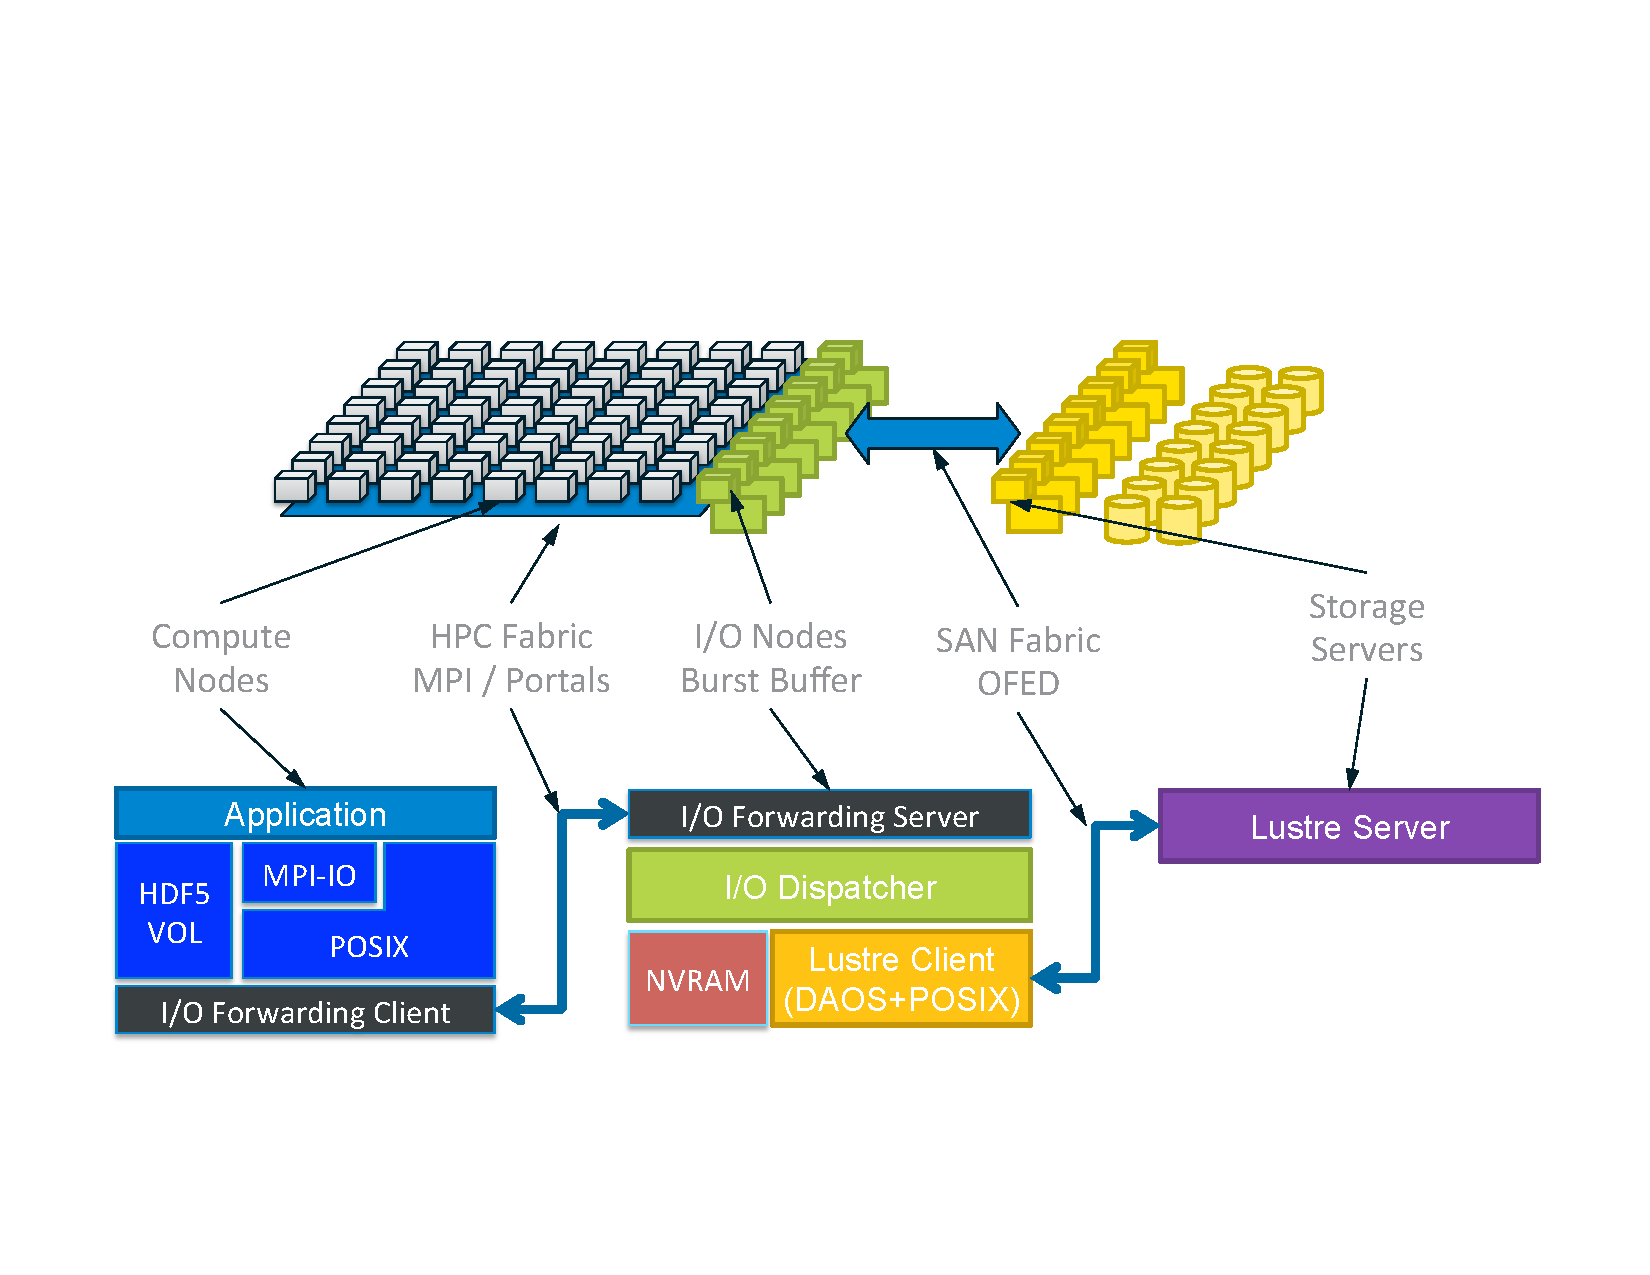
\includegraphics[width=\columnwidth]{images/arch-mapping}
\vspace{-0.15in}
\caption{Target Architecture and Component Mapping}
\label{fig:arch-mapping}
\vspace{-0.15in}
\end{figure}

At a more detailed view, the various layers of the IO stack each contribute
different functionality.  The architecture (Figure~\ref{fig:arch-mapping})
incorporates five layers, some of which have potentially optional components.
The top layer is generally a high level IO library, such as the demonstration
HDF5 library~\cite{hdf5}. It is in dark blue. The intent is to only have
access to the storage stack through such an API to manage the complexity of
working with the lower layers and to enable advanced functionality that would
require more direct user intervention. This layer incorporates the necessary
features for ACGs from a end-user's perspective.

Below the user API is an IO forwarding layer that redirects IO calls from the
compute nodes to the IO dispatching layer (in black).  This IO forwarding layer
is analogous to the function of the IO nodes in a BlueGene machine or the
passive data staging processes demonstrated
previously~\cite{nisar:2008:staging,Abbasi:2009:datatap}. The next two layers
have considerable functionality. The IO dispatcher (IOD) serves as the primary
storage interface for the IO stack (in green) and offers features like Burst
Buffers to insulate the persistent storage array from bursty IO workloads.
Ideally, the IOD layer's functionality can be optional based on available
hardware and compute power provided on the IO Nodes (IONs). Much of the
functionality offered at this layer would shift either up or down the stack as
discussed in detail below. The Distributed Asynchronous Object Storage (DAOS)
layer serves as the persistent storage interface and translation layer between
the user-visible object model and the requirements of the underlying storage
infrastructure. It is intended to be the traditional file system-like
foundation on which everything else is built with no dependence on any
technologies specified above it (in dark pink and yellow). For example, the IOD
layer with or without burst buffers is not required for DAOS to operate
properly.  Instead, the DAOS layer can handle all of the IO operations from the
user API layer, albiet with the potential performance penalty of manipulating
the shared, persistent storage array. At the bottom is the Versioning Object
Storage Device (VOSD) (in purple).  It serves as the interface for storing
objects of all types efficiently for each storage device in the parallel
storage array. Think of this layer as the physical disk interface layer. In
terms of Lustre, this would replace the API on individual storage devices with
an interface friendlier to the containers of objects and transactions/epochs
concepts used in the higher layers.

Along with analysis of the published design documents, a discussion of the
design philosophy representing the overall intent is presented. This
information represents information that may or may not have been written down,
but is the intent of ultimate product.  These ideas are presented to give a
fuller picture of where the project is going rather than dwelling on any
limitations of the published documents. This is most important to illustrate
how different concepts will work across layers since that information is spread
across multiple documents and may lack a cohesive overall view.

The rest of the paper is organized as follows. A brief overview of related work
is presented first in Section~\ref{sec:related}. Section~\ref{sec:end-user}
discusses the programmatic interface end users will see when interacting with
the storage array. This will be discussed in the contect of the HDF5 based
example library used for the functionality demonstration. Section~\ref{sec:iof}
briefly discusses the motivation and proposal for the IO forwarding layer.
Section~\ref{sec:iod} describes the IO Dispatcher layer and the broad
functionality it offers. This will detail the pieces of the layer that are
potentially optional and mention the cross-cutting features discussed in a
later, cross-cutting section. Section~\ref{sec:daos} discusses how the DAOS
layer functions. As with the IOD layer, the cross-cutting features will be
mentioned, but disucssed more fully in the cross-cutting section. The VOSD
layer is disucssed in Section~\ref{sec:vosd}. In particular, the mapping
between the DAOS and VOSD layers are explored as it pertains to the physical
storage. Next is an exploration of cross-cutting features like transactions and
metadata management in Section~\ref{sec:broader}. Since these and other
features are spread across multiple layers, it makes more sense to discuss them
independently once an understanding of the overall structure has been
presented.  A demonstration of the functionality is presented in
Section~\ref{sec:evaluation}. This shows that the prototype system based on the
proposed design can function. The paper is concluded in
Section~\ref{sec:conclusion} with a summary of the broad issues covered in the
paper.

\section{Related Work}
\label{sec:related}

Many projects over the last couple of decades have sought to address some
challenging aspect of parallel file system design. The recent rise of ``Big
Data'' applications with different characteristic IO patterns have somewhat
complicated the picture. Extreme scale machines will be expected to handle both
the traditional simulation-related workloads as well as applications more
squarely in the Big Data arena. This will require some adjustments to the
underlying system for good performance for both scenarios.

The major previous work is really limited to full file systems rather than the
mountain of file system refinements made over the years. A selection of these
other file systems and some features that make it relatively unique are
described below.

Ceph~\cite{weil:ceph} is a distributed object store and file system. It offers
both a POSIX and object interface including features typically found in parallel
file systems. Ceph's unique striping approach uses pseudo-random numbers with a
known seed eliminating the need for the metadata service to track where each
stripe in a parallel file is placed.

PVFS~\cite{carns:pvfs} offers optimizations to reduce metadata server load,
such as a single process opening a file and sharing the handle. It has been
commercialized in recent years as OrangeFS.

Lustre~\cite{braam:lustre-arch} has become the defacto standard on most major
clusters offering scalable performance and fine-grained end-user and
programmatic control over how data is placed in the storage system.

GPFS~\cite{schmuck:gpfs} offers a hands-off approach for providing good
performance for scaling parallel IO tasks and is used extensively by its owner,
IBM.

Panasas~\cite{panasas:architecture} seeks to offer a dynamically adaptive
striping system that detects the need for additional stripes for performance
and adjusts the file layout as necessary.

Other file systems, like GoogleFS~\cite{ghemawat:googlefs}, address distributed
rather than parallel computing and cannot be compared directly. The primary
difference between distributed and parallel file systems is the ability of the
file system to store and retrieve data simultaneously from multiple clients, in
parallel, and treat the resulting collection of pieces as a single object.
Distributed file systems rely on a single client creating a file, but
distributing the set of files across a wide array of storage devices. The
other, popular distributed file system of note is
HDFS~\cite{Shvachko:2010:hdfs} that is distributed as part of Hadoop. These
other file systems are mainly of interest in the context of the ACG features of
FFSIO and will be discussed more in Section~\ref{sec:acg}.

\section{End-User API Layer}
\label{sec:end-user}

Since the proposal specifies a high-level IO API will be the primary end-user
interface for programmatically interacting with the FFSIO stack, the team used
the HDF5 API and leveraged the Virtual Object Layer (VOL) for the initial
design and implementation demonstration. This also serves as a good test
determining what are strictly necessary extensions to an existing IO API to
support the new functionality.  The additional functionality, such as
transactions, can be ignored for legacy implementations, but these applications
will not be able to take advantage of the asynchronous IO support inherent to
the new API.  The additions comprise (Figure~\ref{fig:vol-arch}):

\begin{enumerate}
\def\labelenumi{\arabic{enumi}.}
\itemsep1pt\parskip0pt\parsep0pt

\item
  API extensions to support new functionality provided by the FFSIO project.
  This includes calls for managing asynchronous request lists, performing
  asynchronous operations, creating and managing transactions, end-to-end data
  integrity, and data type and functions to support the ACG functionality more
  efficiently than the current API.

\item\label{item:fs}
  Function shipping from Compute Nodes (CN) to IO Nodes (ION). This provides
  the application developer with the capability of sending computation down to
  the IONs and get back results and perform other operations such as indexing
  and data reorganization for more efficient retrieval.

\item
  Analysis Shipping from CN to IONs or DAOS nodes. This is similar
  to~\ref{item:fs} but instead of returning the result over the network, it
  gets stored on the nodes and pointers to it are returned.

\end{enumerate}

Function and Analysis Shipping are part of the cross-cutting features and are
discussed in Section~\ref{sec:fn-shipping}.

HDF5~\cite{hdf5} has a versatile data model offering complex data objects
and metadata. Its information set is a collection of datasets, groups,
datatypes and metadata objects. The data model defines mechanisms for
creating associations between various information items. The main
components of HDF5 are described below.

\begin{itemize}

\item
  \textbf{File}: In the HDF5 data model, the collection of data items stored
  together is represented by a file. It is an object collection that also
  describes the relationship between them. Every file begins with a root
  group ``/'' serving as the ``starting-point'' in the object hierarchy.

\item
  \textbf{Group}: A group is an object allowing association between HDF5
  objects. It is synonymous with directories in a file system. A group
  could contain multiple other groups, datasets, datatypes or attributes within
  it.

\item
  \textbf{Dataset}: HDF5 datasets are objects representing actual data
  or content. Datasets are arrays with potentially multiple dimensions. A
  dataset is characterized by a dataspace and a datatype. The dataspace
  captures the rank (number of dimensions) and the current and maximum
  extent in each dimension. The datatype describes the type of its data
  elements.

\item
  \textbf{Attribute}: Attributes are used for annotating HDF5 objects. They are
  datasets themselves and are attached to existing objects.

\end{itemize}

\subsection{Virtual Object Layer}
\label{virtual-object-layer}

The Virtual Object Layer is an abstraction mechanism internal to the HDF5
library~\cite{hdf5}. As shown in Figure~\ref{fig:vol-arch} it is implemented
just below the public API. The VOL exports an interface that allows writing
plugins for HDF5 enabling developers to handle data in ways other than writing
to storage in an HDF5 format.  Plugin writers provide an implementation for a
set of functions and are trusted to provide the proper semantics for the new
environment. For example, data staging could be implemented in the VOL layer by
replacing writing to disk in the HDF5 format to sending data to a data staging
area using some messaging mechanism.

For this project, rather than the default writing to disk in the HDF5 format,
the VOL is used to interact with the IOD layer and the different concepts it
offers without requiring all of the functionality be exposed to users. For
example, the containers and objects concept is transparently mapped to the
files and datasets existing HDF5 users are familiar with.  This reduces the
difficulty porting applications to the new IO stack.

\begin{figure}[htbp]
\vspace{-0.10in}
\centering
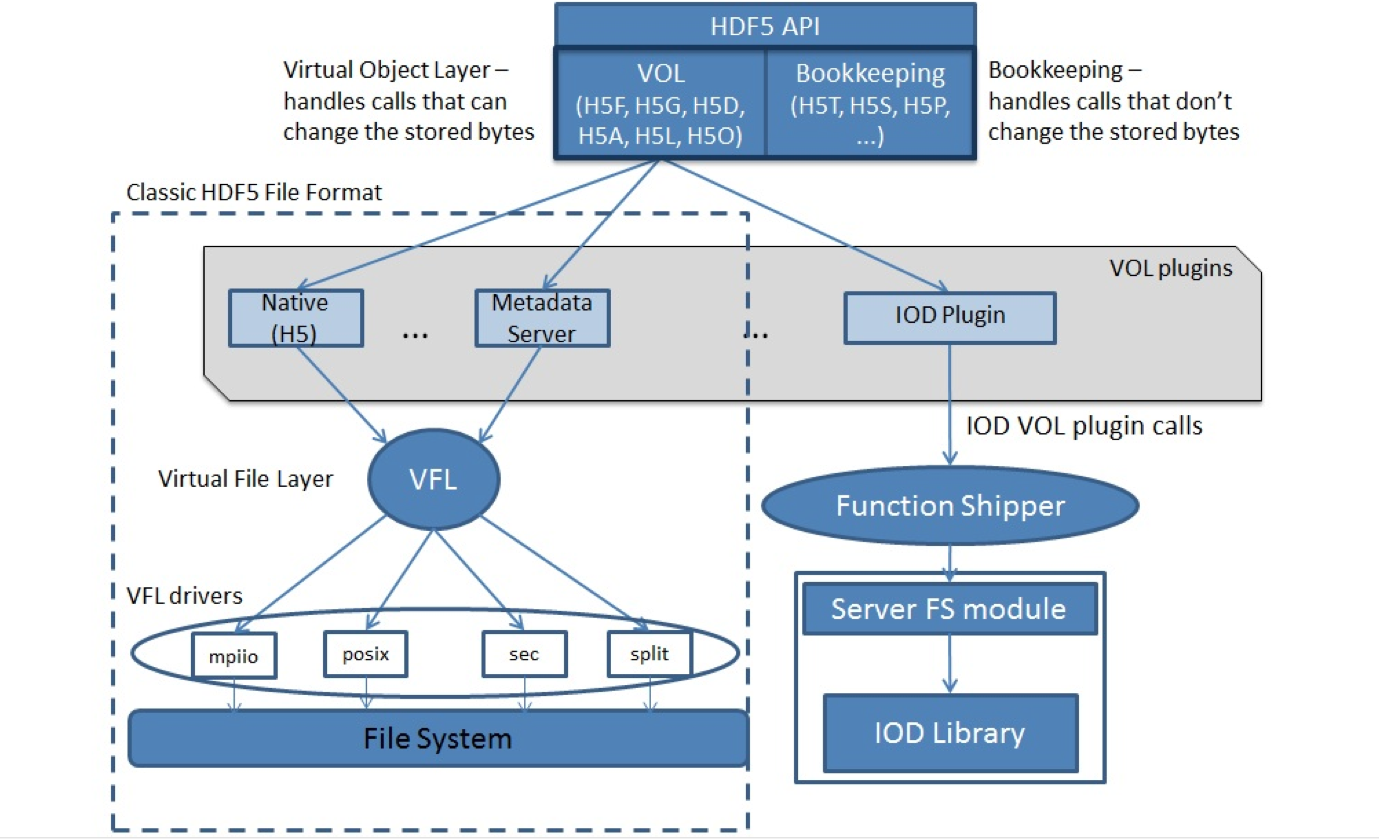
\includegraphics[width=\columnwidth]{images/vol-arch.png}
\vspace{-0.10in}
\caption{Architectural view of the VOL abstraction mechanism}
\label{fig:vol-arch}
\vspace{-0.10in}
\end{figure}

The IOD VOL plugin serves as the bridge between HDF5 and the IOD or DAOS Layer
(Figure~\ref{fig:vol-arch}). The application calls the HDF5 library while
running on the system's compute nodes. Using the VOL architecture, the IOD VOL
plugin uses a function shipper (RPC library) to forward the VOL calls to a
server component running on the IO nodes (IONs). This function shipping is the
IO Forwarding Layer discussed briefly in Section~\ref{sec:iof}. Once the calls
arrive at the IO nodes, they are translated into IO Dispatcher (IOD) API calls
and executed at the IONs.

\subsection{HDF5 to FFSIO Mapping}
\label{sec:hdf-to-ffsio}

Since HDF5 has traditionally offered an interface focused on files and the
internal data types, such as datasets, these concepts must be mapped onto the
proposed FFSIO data storage concepts. This mapping is shown in Table~\ref{tab:mapping}

\begin{table}[ht]
    \vspace{-0.10in}
    \centering
    \caption[HDF5 to FFSIO Mapping]{HDF5 Data Model to FFSIO Data Model Mapping}
    \bigskip
    \vspace{-0.15in}

    \begin{tabular}{|r|r|}
\hline
HDF5 & FFSIO\\
\hline
file & container \\
dataset & array \\
group & key-value store \\
attribute(s) & key-value store \\
\hline
    \end{tabular}
    \label{tab:mapping}
\end{table}

In Section~\ref{sec:iod} below, the FFSIO types are described in more detail.

\section{IO Forwarding Layer}
\label{sec:iof}

The IO Forwarding layer offers a mechanism to reduce the concurrency impact of
the massive process count on the storage stack. A current trend mixing MPI with
a threading library like OpenMP is addressing the same issue, but limited to
handling the parallelism on a single node rather than multiple nodes. Projected
extreme scale platforms will have far fewer storage stack end-points per
compute process in which to receive requests and data. By reducing the number
of simultaneous requests, delays can be reduced. This has been demonstrated for
the file open operation with Lustre~\cite{lofstead:2009:adaptable} and to some
degree for accessing the storage devices
themselves~\cite{lofstead:2010:io-variability}.  The BlueGene platform
incorporated dedicated hardware to perform this role. The proposed
functionality for this layer, beyond managing the number of connections to the
IOD layer, is to implement function shipping from the compute nodes to the IO
nodes.

For the basic HDF5 calls, this will work the same as how the Nessie
staging~\cite{lofstead:2011:nessie-staging} shifted the collective IO data
rearrangement calls to a reduced number of processes. The prototype
implementation will only support accessing functionality already deployed to
the IO nodes through an RPC mechanism. This initial implementation will use
Mercury~\cite{Soumagne:2013:mercury} to access the remote functionality. For
dynamically defined functions, a different system will be required leveraging
something like C-on-demand~\cite{abbasi:2011:c-on-demand} or some other dynaimc
deployment and compilation or an interpreter system.

\section{IO Dispatcher Layer}
\label{sec:iod}

Strictly speaking, the IO Dispatcher layer and included functionality, such as
burst buffers, is optional. All of the functionality, such as function and
analysis shipping, transaction management, and managing asynchronous data
movement can be handled by other portions of the stack. For an extreme scale
platform, the IOD layer will be an essential pressure relief valve for the
underlying persistent storage layer. By making it optional, the proposed stack
can be deployed more easily on smaller clusters or for those with more
constrainted budgets. For simplicity, the rest of this section will describe a
full stack including all of the proposed IOD components.

The core idea for IOD is to provide a way to manage IO load that is
separate from the compute nodes and the storage array. Communication intensive
activities, such as data rearrangement, can be moved to the IOD layer
reducing the number of participants and message count. IOD has three main
purposes. First, the burst buffers work as a fast cache absorbing write
operations that then trickles out to the central storage array. It can also
be used to retrieve objects from the central storage array for more efficient
read operations and offers data filtering to make client reads more efficient.
Second, it offers the transaction mechanism for controlling data set visibility
and to manage faults that could expose an incomplete or corrupt data set to
users. These transactions are local to the IOD layer until persisted to the
DAOS layer eliminating the need for burdening the persistent storage with
transient data.  Third, data processing operations can be placed in the IOD.
These operations are intended to offer functionality like data rearrangement
and filtering prior to data reaching the central storage array.

While these ideas are not necessarily new, they are new twists on best of class
efforts for these technologies. For example, offloading the collective
two-phase data sieving from the compute nodes to reorganize data has proven
effective at reducing the total time for writing data due to fewer participants
involved in the communication patterns~\cite{lofstead:2011:nessie-staging}.
Beyond these broad items, there are many important details some of which are
examined in more detail below.

\subsection{FFSIO Data Model Types}
\label{sec:data-model}

With the shift from a directories and stream-of-bytes files model to the
container and object model, some description is required to better understand
how these concepts are being used as well as the raw benefits.

\subsubsection{Container}
As mentioned above, the concept of a container is similar to that of a file in
a traditional file system. However, rather than being in a directory structure,
each container essentially is stored in a hash-space allowing direct access to
any container without regard to the current organizational context of the
file system. For example, there is no need to navigate a directory hierarchy
to name a particular container.

Functionally, a container plays the same role as a file in that it holds a
collection of presumably related data intended to be accessed and manipulated
as a unit. Since this is extended from HDF5 files, the container could also be
viewed as a directory tree of objects where each directory entry specifies
either a sub-directory (group) or some data or attribute.

\subsubsection{Key-Value Store}
This is the base type for the container. Since the container represents
something akin to HDF5 files, everything is stored within a hierarchical
namespace. The root namespace is represented by the base key-value store and
contains a list of all of the objects for this portion of the namespace as well
as additional key-value objects representing sub-groups for the hierarchy. Each
of those key-value store objects works identically.

Attributes are stored in a key-value store object, but use the
multi-dimnensional array and blob objects to store the values for the
attributes.

\subsubsection{Multi-Dimensional Array}
By treating arrays as a special case separate from blobs, additional
opportunities are enabled. For example, by knowing that an object is an array,
proper slicing of that array onto IO nodes can be done without involving higher
levels of the IO stack.

\subsubsection{Blob}
All other data is stored as a stream-of-bytes without regard to the actual
data type.

\subsection{Multi-Dimensional Array Data Distribution}

For both IO performance and to aid in analysis and other data processing, the
multi-dimensional array object can be split across multiple IO nodes. Each
piece of this array is called a {\em shard}.  The idea of sharding is to store
a logically complete portion of a data set on a single storage target. This is
similiar in concept to the HDF5 hyperslab.  The FFSIO stack supports sharding
the data in the default or some other structured way as well as ``re-sharding''
based on application needs. For example, reordering the data so that a
different dimension is the ``fast'' dimension may greatly improve the
performance of a subsequent data analytics task. A common scenario where this
is common is a Fortran code (column-major) writes data for a C code (row-major)
to analyze.  The IOD API supports the following sharding strategies:

\begin{itemize}
\itemsep1pt\parskip0pt\parsep0pt
\item
  \textbf{contiguous}. fixed chunking, distributed in a round-robin
  fashion accross the IO nodes.
\item
  \textbf{chunked}. same as above but with irregular (sparse) chunking.
\item
  \textbf{user-defined}. either contiguous or chunked, but user specifies
  where to place each individual shard.
\end{itemize}

It is possible to request the transformation of an object's physical
layout to other formats, having multiple copies of the same objects in
multiple formats if desired. Also, the user can pre-fetch objects from
the storage cluster into the IO nodes or read them directly from the
storage cluster. At the semantic level (HDF5), indices can be created
for datasets resulting in being able to read through an index instead of
directly from the base array.

All of these distinct alternatives result in having many different ways for
executing the same analysis task.  In the subsequent discussions, we consider
only data-movement optimization, i.e., sending the analysis code as close as
possible to the data. In practice, this means we focus on identifying sharding
of datasets and execute code accordingly over the appropriate shards.

\subsection{IO Nodes}
IOD processes are hosted on the IO nodes that interface a general compute area
with the storage array. The IO nodes handle requests forwarded by the
scientific applications, potentially integrate a tier of solid-state devices to
absorb the burst of random or high volume operations, and organize/re-format
the data so that transfers to/from the staging area from/to the traditional
parallel file system can be done more efficiently. It also has the capacity to
execute analysis on data recently generated by simulation applications running
at the compute nodes, but not persisted to the storage array. As the data
arrives, re-organization and data preparation can be applied in order to
anticipate the execution of analytical tasks.

\begin{figure}[htbp]
\centering
\vspace{-0.10in}
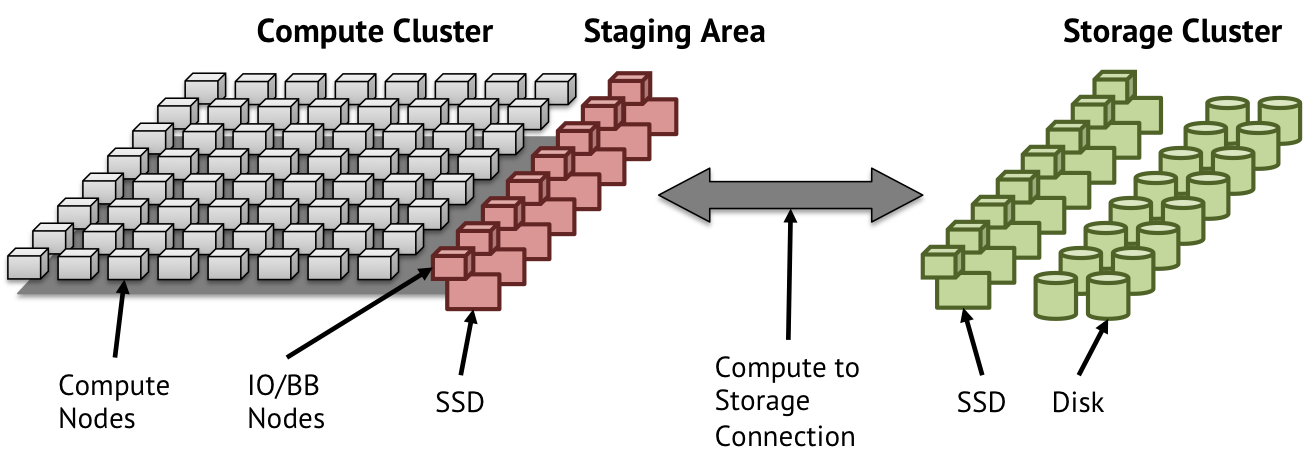
\includegraphics[width=\columnwidth]{images/exa-arch.png}
\vspace{-0.20in}
\caption{Exascale Architecture}
\label{fig:exa-arch}
\vspace{-0.10in}
\end{figure}

A common configuration for this type of deployment is shown in
Figure~\ref{fig:exa-arch}. The designated IO nodes (IONs) are connected to the
compute nodes (CNs) through the same fast fabric (e.g., InfiniBand) while the
connection to the external storage cluster is through a secondary, slower
channel (e.g., 10Gb Ethernet). By providing additional storage on the IO nodes,
such as SSDs, these nodes are capable of better regulating the IO pressure on
the underlying storage array better than simple forwaring gateways. For this
project, using something like SSDs on the IO nodes is termed a {\em Burst
Buffer} and is disucssed below.

\subsection{Burst Buffers}
\label{sec:burst}

The idea of burst buffers were initially explored in the context of data
staging~\cite{abbasi:2007:datatap,Abbasi:2009:datatap,nisar:2008:staging,zheng:2010:predata}.
These initial designs all use extra compute nodes to represent the data storage
buffer given the lack of any dedicated hardware support for this functionality.
The desired outcome of these initial studies is to motivate how such
functionality might be incorporated and the potential benefits.  Later, these
concepts were proposed to be incorporated into the existing IO stack
architecture~\cite{nowoczynski:2008:zest,bent:2012:challenges,bent:2012:burst-buffer}.

In the case of the written IOD design, it describes a fixed-sized staging area
that is partitioned on a per-application basis. As part of an application
being deployed into the platform, each application will be allocated a fixed
number of IO nodes for exclusive use during the application run. This provides
guarantees about how much burst buffer space and processing capability will be
available for the applications.

Future work will generalize this model to potentially support dynamic IO node
allocation and examine the possibility of oversubscription. It will be strictly
necessary to consider shared IO nodes for cases where the number of deployed
applications exceeds the number of IO nodes.  This first phase focuses on
extreme scale application runs that use the vast majority of a platform rather
than a capacity cluster where end-to-end performance is a lesser concern.

\noindent\textbf{Design Philosophy}

The burst buffers design, as presented in the IOD documents, limits the
placement of the function operators and SSD buffers to the IO nodes. The
limitations of this design are acknowledged and the intent is to ultimately
spread the IOD layer from the IO nodes into the compute area as well.  This is
intended both to help address the limitations of the IO bandwidth and compute
capability of these few nodes for data processing, but also to take advantage
of new layers in the storage hierarchy. By incorporating NVRAM into compute
nodes, new options for buffering data prior to being moved to centralized
storage become available and addresses potential concerns about SSD
performance. For example, including a small amount of Phase Change memory into
many or most compute nodes offers a way to move data outside of both the
compute and IO path for data and communication intensive operations. Other
projects~\cite{zheng:2010:predata} have shown this will have value, but the
cost will have to be considered as part of the overall platform budget. This
lessens the impact of some operators while offering additional options for
places to store data.

Burst buffers being optional is a high level goal, but not considered in detail
within the phase one design. If there is no burst buffer, all of the advanced
functionality proposed for the IOD layer would have to work against the DAOS
layer instead. For example, function shipping assumes it will operate on fast,
local data within the IOD layer rather than against the globally shared DAOS
layer. With the additional desire to support using compute node resources for
these operations, serious work will be required to make a fully functional
end-to-end IOD layer implementation for a production system.

\section{DAOS Layer}
\label{sec:daos}

The Distributed Asynchronous Object Storage layer serves as the traditional
parallel file system interface layer for the storage devices. This is the
consistent, global view of the underlying devices represented in this stack
by the VOSD layer.

This is the layer where the container/object model is translated into the
physical storage requirements dictated by the physical storage underneath (the
VOSD layer). The two key design elements of this layer are the handling of
epochs and the mapping of conatiners and objects to the underlying storage.

There is a bit of a terminology shift between the IOD layer and the DAOS
layer. For the IOD layer, a shard represents a portion of an object that is
spread across potentially multiple IO nodes. For the DAOS layer, a shard
represents the portion of a container that is spread across potentially
multiple physical storage devices.  The physical storage devices are
represented by the VOSD layer described in Section~\ref{sec:vosd}.

While transactions at the HDF5 and IOD layer use the same term, at the DAOS
layer the terminology shifts. Instead of transactions, the term {\em epochs}
is used instead. Rather than attempting to introduce confusion, this is intended
to help clarify how these concepts are used at different layers of the FFSIO
stack. In the HDF5 and IOD layer, every operation has a transaction that may
or may not ultimately be persisted to the DAOS layer. When a transaction is
persisted to DAOS, it is termed an epoch to reflect that this is a persistent
version of the container. For simplicity the epoch ID is the same as the
transaction ID that was persisted.

The process of persisting a transaction to an epoch involves a process called
``flattening''. Since this stack uses a copy-on-write approach to reduce the
space requirement for new versions of existing files, when a transaction is
persisted to a DAOS epoch, all of the changes between the last epoch and the
current epoch must be combined into a single entry. The process of combining
the changes from a series of transactions into a single update for an epoch
is termed flattening.

The current implementation has the DAOS layer map the container/object data
model onto a directory/file data model used for most existing file systems.
Should a fully object-based file system be deployed at the VOSD layer, this
mapping would be unnecessary. The current projections suggest that a standard
POSIX-like file system will likey be used at the lowest level on each storage
device requiring the mapping at some level. To perform this mapping, DAOS
considers the following.

Each container is represented by a directory on some storage device containing
symbolic links to all of the shards it contains and maintains the epoch ID.
In particular the Highest Committed Epoch (HCE) is an important concept for
quickly identifying which version of a shard to retrieve and to block writes to
older epochs since those have been committed.

Overall, the DAOS layer serves as the shared persistent storage interface for
the IO stack. In the case of a data center-wide storage array, the DAOS layer
would be shared across all of the platforms with the upper layers being local
to each individual platform.

To address consistency issues between platforms, containers at the DAOS layer
must know of every transaction. To address this, a container is updated every
time a new transaction is created for it and closed or aborted. This ensures
that if multiple platforms are writing to the same container sequentially that
they will not have conflicts in the highest transaction number. The FFSIO stack
does not support multiple applications from the same or different platforms
using a shared DAOS layer to write to the same container at the same time.

\section{VOSD Layer}
\label{sec:vosd}

The Versioning Object Storage Device (OSD) layer operates as the interface for
each persistent storage device used to support the parallel storage array. In
the purest form, it uses a local file system to arrange storage of objects that
represent parts of the higher level objects in containers.

The base level implementation continues the space optimization of only storing
changes for new versions by using a copy-on-write file system. The prototype
uses ZFS~\cite{zhang:2010:zfs} for the known stability and integration with
Lustre. In a production version of the FFSIO stack,
btrfs~\cite{rodeh:2013:btrfs}, The Linux B-Tree File System, given its
open-source backing and GPL licensing, is a likely long-term choice.

At a more detailed level, the design for VOSD is an increment beyond the
current Lustre Object Storage Device design to incorporate the idea of shards
and the versioning aspects of transactions/epochs. For every DAOS shard, the
VOSD has information for storing and accessing the currently commited version,
the Highest Committed Epoch, as well as a staging dataset represeting the
next version of the object being stored. Both of these are combined in a shard
root.

For data integrity, an intent log is maiained as part of the underlying file
system enabling fault recovery.

Beyond the functionality to incorporate and expose the copy-on-write nature
of the underlying file system and the semantics for storing and processing
shards and their associated epochs, this is largely an evolution of the
existing Lustre OSD layer.

\section{Broader Design}
\label{sec:broader}

Several concepts crosscut many of these layers and are best described in a
single location. For example, transactions and epochs are visible from the
user API level down into the VOSD layer. While each layer affects the concept,
it is best to look at it across all of the layers.

In the subsections that follow, we examine transactions and epochs, metadata
management, function and analysis shipping, and the aribtrary connected graphs
support.

\subsection{Transactions and Epochs}
\label{sec:transactions}

As mentioned above, the transaction mechanism manifests in two forms. From the
user level down through the IOD layer, they are called transactions and are
used to judge whether or not a set of distributed, asynchronous modifications
across a set of related objects is complete or not.  It is also used to control
access by treating the transaction ID of committed transaction as a version
identifier.  At the DAOS layer and below, they are called epochs and represent
persisted (durable) transactions from the IOD layer. Each of these offers
different functionality, but are connected as is explained below.

\subsubsection{Transactions}
To understand how transactions are used in the IOD layer, some terminology and
concepts must be explained first. At the coarsest grain level is a container.
Each container provides the single access context through which to access a
collection of objects. Transactions are the way that a series of modifications
to the objects within a container are treated atomically. Conceptually,
containers corresponds to a something akin to an HDF5 file in a traditional
file system. The objects in each container represent different data within a
file.  The three initially defined object types are key-value stores,
multi-dimensional arrays, and blobs.  The easiest way to understand these types
is to evaluate these from the perspective of an HDF5 file, the initial user
interface layer. The key-value store represents a collection of attributes or
groups. The array represents a potentially multi-dimensional array.  The blob
represents a byte stream of arbitrary contents.  The fundamental difference
between an array and a blob is that the array has metadata specifying the
dimension(s). At the physical layer within the IO nodes, all of these objects
may be striped across multiple IO nodes.  Given this context, the transactions
come in two forms.

First is a single leader transaction where the IOD manages based on calls from
a single client. The underlying assumption is that the client side will manage
the transactional operations itself and the single client is capable of
reporting to the IOD how to evolve the transaction state. 

The second form is called multi-leader and has the IOD layer manage the
transactions. In this case, when the transaction is created, a count of clients
is provided to the IOD layer. As clients commit their changes to the container,
the reference count is reduced. Once the count reaches 0, the transaction is
automatically committed.

\noindent\textbf{Design Philosophy}

Undocumented, but inherent in the design of these transactions is how faults
are detected. The initial design assumes the current Lustre fault detection
mechanism that can determine if a process or node is no longer reachable. This
detection happens at the DAOS layer and when a fault is detected, the rollback
process is pushed up to the IOD layer for all non-persisted or non-committed
transactions. This defines how a fault will be detected and what will trigger a
passive fault recovery (i.e., transaction abort).

There are two steps for beginning a transaction on a container. The first step
is for one or more process to open the container. This handle can be shared
eliminating the need for every participating process to hit the IOD layer to
open the file. The second step is a call to determine how many leaders will
participate in the transaction. In the single leader case, there is no
aggregation of success/fail statuses to determine the final transaction state.
Instead, it is assumed that the client will fully manage the transaction. In
the multi-leader model, some subset from 2 to $n$ where $n$ is the count of all
processes, declare themselves a leader for this container operation to the IOD
layer. Any number of processes can participate in modifying container without
regard to whether or not they are a leader. Once each leader has finished, with
the assumption that any clients they may be responsible for are finished as
well, the IOD layer aggregates those responses to either commit or abort the
transaction.

Ultimately, with the passive detection of faults for transaction leaders, the
transaction mechanism can work very well. A mostly unstated restriction that is
being relaxed is that every sequential transaction on a container is considered
dependent on the earlier transaction. Should one output be delayed and the
subsequent five succeed, when the delayed process finally fails, all six
transactions are rolled back. The thought of using this mechanism to store
subsequent checkpoint outputs in the same container to both save space, but not
care if one fails, cannot work in the current form. This has been acknowledged
and is being relaxed requiring a new parameter to the creation of a transaction
determining if it will be dependent or not.

\subsubsection{Epochs}
The Epoch mechanism differs from transactions. Instead of focusing on when a
particular output is complete, an epoch represents incremental persisted
container copies.  To simplify the mapping between an IOD transaction and the
DAOS epochs, when an IOD transaction is persisted to DAOS, the IOD transaction
ID is the used as the epoch ID. The key difference is that at the DAOS layer,
some transaction (epoch) IDs will not be represented with data since not all
IOD transactions are necessarily persisted. Maintaining this ID continuity is
critial for multiplatform use. Since the shared point is the DAOS layer, any
user adding a new version to a file must be able to determine the most recent
transaction ID no matter from where the container was updated last.

\subsection{Metadata Management}
Metadata management has been a perennial challenge for parallel storage
systems.  Eliminating metadata management as a special case and instead
treating it just as data is a central design goal of the Fast Forward project.
This is a hybrid approach to metadata management that is half-way between
providing no inherent metadata support and having a fully integrated, but
separate metadata management system.

Eliminating metadata as a core component of a file system is not new. It has
been explored as part of the Light Weight File Systems
project~\cite{oldfield:lwfs}. In LWFS, the metadata service is explicitly
limited to a user task with the storage layer limited to data
storage/retrieval, authorization, and authentication. This approach proved
workable. Using this hybrid approach is less common~\cite{weil:2006:ceph} and
introduces other issues.

IOD and DAOS both share a philosophy that they will have to maintain the
metadata about how the physical pieces of the logical objects are striped and
where they are placed. The primary metadata management is done at the DAOS
layer with the IOD layer relying on the DAOS layer for all authoritative
information about containers and objects. The only place where the IOD layer
manages metadata for itself is to manage how the different objects are striped
across the IO nodes.

\noindent\textbf{Design Philosophy}

While the metadata design is not fully defined, there are a few things that
are intended. For example, there will be a standard, well-known container that
is the system metadata. This includes the list of all other containers. This
container is treated like any other data in the system and striped as
appropriate. Unfortunately, this still couples the metadata to a single object
that must serialize access. If the metadata, including information about
striping and other data layout operations were separated completely from the
data path, more scalable throughput could be achieved. The real challenge of
this is introduced by the IOD, DAOS, and VOSD layers collectively. Each of
these requires some different metadata storage and the migration is transparent
to the user.  Supporting fully independent metadata with this model is
difficult. Serious thought on how to do this effectively outside the data path
will be considered for phase two.

\subsection{Function and Analysis Shipping}
\label{sec:fn-shipping}

A client/server architecture is implemented for the Compute Node-IO Node
communication model.  Every ION runs an IOFSL (IO Function Shipping Layer)
server. The IOFSL client is integrated into the HDF5 library which runs on each
CN. A client can forward requests to any number of IONs. Every IO operation
issued by HDF5 is asynchronously shipped to the IOFSL server and asynchronously
executed. As it is currently implemented, the only functionality that can be
``shipped'' already exists on the IONs and is activated using RPC calls. This
will be re-evaluated for phase two to provide more dynamic functionality.

\subsection{Arbitrarily Connected Graphs}
\label{sec:acg}

What people popularly consider Big Data applications fall into two broad
categories. First, data processing tasks that can fit into the MapReduce model
where data is tagged and sorted to discover relationships. These sorts of
applications only require scale out rather than scale up. Scaling out requires
replicas to process data simultaneously, but do not need to coordinate for that
data processing. Scaling up, what scientific simulations do, requires sometimes
serious coordination between the processes for any of them to succeed. In the
middle are graph applications that, with some replicated data, can be made to
fit reasonably well into the MapReduce model. The challenge is having access to
the edge and vertex lists effectively to build partitions for independent
processing. GraphBuilder~\cite{Jain:2013:GraphBuilder} is a tool to generate
effective graph paritions reducing the load for using MapReduce to process
graph data sets. GraphLab~\cite{Low:2012:GraphLab} offers a way to process
these graphs efficiently for parallel platforms using a minimum of
communication. Using these tools as motivators, changes to the HDF5 interface
and the underlying storage infrastructure is proposed.  The following
illustrates the architecture of both frameworks:

\begin{figure}[htbp]
\centering
\vspace{-0.10in}
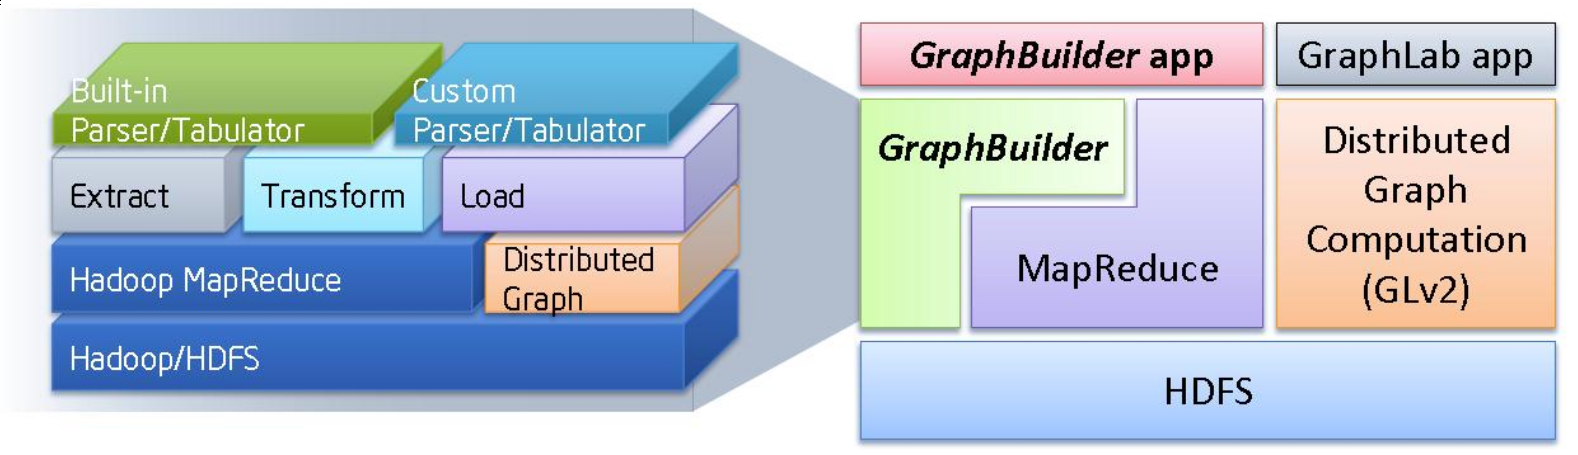
\includegraphics[width=\columnwidth]{images/graphlab-and-graphbuilder.png}
\vspace{-0.30in}
\caption{GraphLab and GraphBuilder stacks}
\label{fig:graphlab-graphbuilder}
\vspace{-0.10in}
\end{figure}

In order to make both of these tools work on top of the exascale stack, they
both have to be modified. After these modifications are implemented,
GraphBuilder will be able to write the partitioned graph in the newly proposed
HDF5 files which will thus be stored in the IOD nodes (or IONs) in a
parallel-optimized way. On the GraphLab side, HDF5-awareness will allow
the library to perform at high speeds by benefiting from the new
features, such as the function shipping. In general both frameworks will be
modified so that calls to HDFS-based formats are replaced by the proposed HDF5
equivalents. This is referred to as the HDF Adaptation Layer or HAL and will
provide, from the GraphBuilder/GraphLab point of view:

\begin{itemize}
\itemsep1pt\parskip0pt\parsep0pt
\item
  capability for storing the newly proposed HDF5 format
\item
  association of network information to vertices/edges
\item
  shipping computation to the IONs
\item
  asynchronous vertex updates
\item
  efficient data sharing ammong CNs
\item
  computation over versioned datasets
\end{itemize}

The initial phase of this project has determined the necessary changes in the
HDF5 format to support these features. These identified features will be
proven during phase two with a demonstration of GraphBuilder and GraphLab.

\section{Demonstration}
\label{sec:evaluation}

This stack has an early prototype implementation intended to test concepts
rather than performance and scalability. It has focused on examining the
interaction of the different APIs for each layer to flesh out any detailed
requirements or concerns that may have been missed in the conceptualization of
this IO stack. To demonstrate the viability of the IO stack described in this
paper, we show some very early performance results from the untuned prototype.

All of the tests are performed on the Buffy Cray test cluster at Los Alamos
National Laboratory. It consists of 84 nodes each with dual, 8 core Intel
Xeon ES-2670 CPUs at 2.6 GHz and 32 GB RAM. The inteconnect is Cray Gemini.
The storage array are three sets of SSD-based lustre file systems.

We run two different sets of tests. The first set in
Figure~\ref{fig:eval-hosts} show the reading and writing performance for
different number of hosts. Each read or write is 4 GB against the x-axis number
of hosts. The second set in Figure~\ref{fig:eval-size} show the performance of
reading and writing different sizes for 56 clients, the smallest client count
when performance stabilizes in the number of hosts tests.  The performance of
both of these tests are reported to give a very rough idea of the overhead that
might be involved. Rather than a true overhead, this should be considered the
maximum overhead that should be expected once an optimized, fully functional IO
stack is deployed without relying on translating to an underlying parallel file
system. 

\begin{figure*}[htbp!]
\centering
\vspace{-0.10in}
\subfigure[Write Hosts]{\label{fig:write-hosts}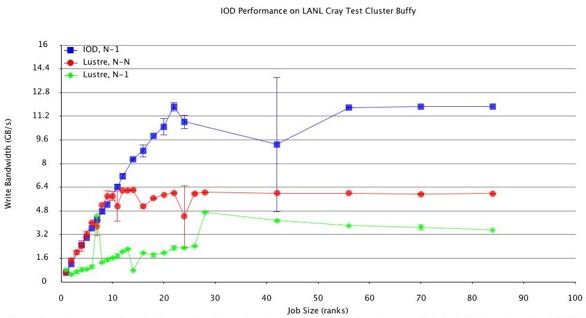
\includegraphics[width=\columnwidth]{images/write-hosts.png}}
\subfigure[Read Hosts]{\label{fig:read-hosts}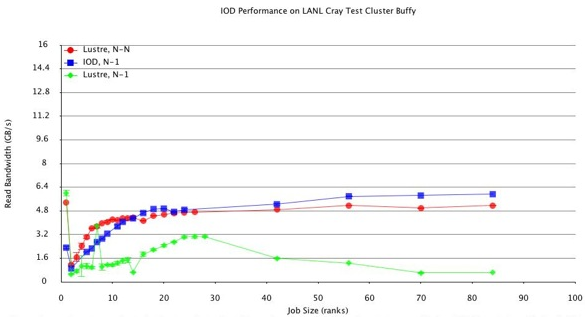
\includegraphics[width=\columnwidth]{images/read-hosts.png}}
\vspace{-0.10in}
\caption{Functionality Demonstration Validation for Number of Hosts}
\label{fig:eval-hosts}
\vspace{-0.05in}
\end{figure*}

\begin{figure*}[htbp!]
\centering
\vspace{-0.10in}
\subfigure[Write Size]{\label{fig:write-size}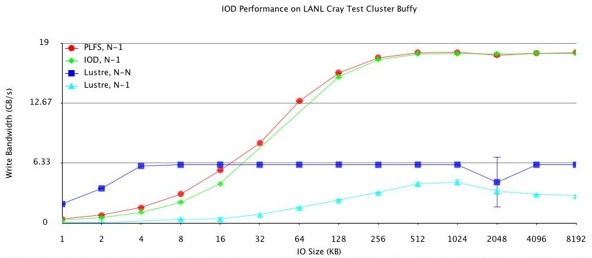
\includegraphics[width=\columnwidth]{images/write-size.png}}
\subfigure[Read Size]{\label{fig:read-size}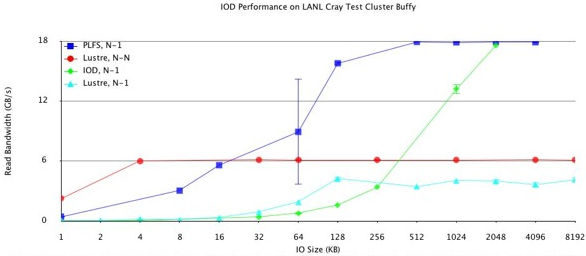
\includegraphics[width=\columnwidth]{images/read-size.png}}
\vspace{-0.10in}
\caption{Functionality Demonstration Validation for Data Sizes}
\label{fig:eval-size}
\vspace{-0.05in}
\end{figure*}

\section{Conclusions}
\label{sec:conclusion}

The Fast Forward Storage and IO Stack project has designed a good first pass at
addressing the requirements for an extreme scale data storage mechanism.  By
prefering a high level user API like HDF5 rather than using the POSIX
interface, more advanced functionality can be incorporated with less end-user
impact. The introduction of the IOD layer with buffering will absorb the
difference between the compute node IO demands and the available bandwidth in
the storage array. With DAOS supporting translating the container and object
model to the underlying storage options, different storage technologies can be
deployed over time.

With the overall stack design a prototype implementation complete, refinements,
such as fault detection and recovery, can be designed and tested.  These and
other activities for phase 2 will ultimately generate what is likely to be the
next generation storage stack for extreme scale platforms.

\section{Acknowledgements}


\includegraphics[scale=0.07]{logos/doe_logo}

\includegraphics[scale=0.30]{logos/snl_logo}

\includegraphics[scale=0.35]{logos/nnsa_logo}
Sandia National Laboratories is a multi-program laboratory managed and operated
by Sandia Corporation, a wholly owned subsidiary of Lockheed Martin
Corporation, for the U.S. Department of Energy's National Nuclear Security
Administration under contract DE-AC04-94AL85000.

\bibliographystyle{abbrv}
\bibliography{paper}

\vfill\eject

\end{document}
